\documentclass[../Thesis.tex]{subfiles}
\begin{document}
	
	\section{State of the Art Review}
	\label{sec:state_of_the_art_review}
	
	Traditional imperative solutions for solving the graph edit distance (GED) problem have been effective for graphs of modest size, utilizing explicit algorithms that compare graphs node by node and edge by edge through combinatorial techniques. However, as the number of nodes in the graph increases, the complexity of these methods grows exponentially, leading to significant scalability issues. In such scenarios, imperative solutions often become impractical, requiring an inordinate amount of time to compute the GED. This challenge is particularly critical in domains like bioinformatics, social network analysis, and cheminformatics, where large-scale graphs are common.
	
	To address these scalability challenges, recent research has pivoted towards leveraging artificial intelligence (AI) models. AI-based approaches offer more robust and scalable solutions by learning patterns and features from graph data, significantly reducing computation times and improving accuracy. This section reviews some of the prominent AI-based models that have advanced the state of the art in GED computation.

	The timeline of notable advancements in this field starts with \textit{SimGNN} in 2019 \cite{simgnn__a_neural_network_approach_to_fast_graph_similarity_computation}, the first approach to utilize neural networks for computing GED. Subsequent models have built upon this foundation, progressively enhancing the accuracy and efficiency of GED computation. This review covers developments from SimGNN to the latest contributions in 2023, culminating in the VLDB paper introducing \textit{GedGNN} \cite{computing_graph_edit_distance_via_neural_graph_matching}. These models collectively represent significant strides in utilizing AI to overcome the limitations of traditional GED computation methods.
	
	\subsection{Timeline}
	\label{subsec:timeline}
	
	2019, \textit{SimGNN: A Neural Network Approach to Fast Graph Similarity Computation} \cite{simgnn__a_neural_network_approach_to_fast_graph_similarity_computation}: Introduces SimGNN, addressing graph similarity computation using neural networks. It features a learnable embedding function, an attention mechanism to emphasize important nodes, and a pairwise node comparison method, achieving better generalization and computational efficiency compared to baselines.
	
	2020, \textit{Learning Graph Edit Distance by Graph Neural Networks} \cite{learning_graph_edit_distance_by_graph_neural_networks}: Introduces a framework combining deep metric learning with traditional approximations of graph edit distance using geometric deep learning. The approach employs a message passing neural network (MPNN) to capture graph structure and compute graph distances efficiently, showing superior performance in graph retrieval and competitive results in graph similarity learning.
	
	2020, \textit{Combinatorial Learning of Graph Edit Distance via Dynamic Embedding} \cite{combinatorial_learning_of_graph_edit_distance_via_dynamic_embedding}: Introduces a hybrid approach for solving the GED problem by integrating a dynamic graph embedding network with an edit path search procedure, enhancing interpretability and cost-efficiency. The learning-based A* algorithm reduces search tree size and saves time with minimal accuracy loss.
	
	2021, \textit{Graph Partitioning and Graph Neural Network-Based Hierarchical Graph Matching for Graph Similarity Computation} \cite{graph_partitioning_and_graph_neural_network_based_hierarchical_graph_matching_for_graph_similarity_computation}: Introduces PSimGNN, which partitions input graphs into subgraphs to extract local structural features, then uses a novel GNN with attention to map subgraphs to embeddings, combining coarse-grained interaction among subgraphs with fine-grained node-level comparison to predict similarity scores.
	
	2021, \textit{Noah: Neural Optimized A* Search Algorithm for Graph Edit Distance Computation} \cite{noah__neural_optimized_a*_search_algorithm_for_graph_edit_distance_computation}: Introduces Noah, combining A* search algorithm and Graph Path Networks (GPN) for approximate GED computation. Noah learns an estimated cost function using GPN, incorporates pre-training with attention-based information, and adapts an elastic beam size to reduce search complexity.
	
	2021, \textit{Learning Efficient Hash Codes for Fast Graph-Based Data Similarity Retrieval} \cite{learning_efficient_hash_codes_for_fast_graph_based_data_similarity_retrieval}: Introduces HGNN (Hash Graph Neural Network), a model designed for efficient graph-based data retrieval by leveraging GNNs and hash learning algorithms. HGNN learns a similarity-preserving graph representation and computes compact hash codes for fast retrieval and classification tasks.
	
	2021, \textit{More Interpretable Graph Similarity Computation via Maximum Common Subgraph Inference} \cite{more_interpretable_graph_similarity_computation_via_maximum_common_subgraph_inference}: Introduces INFMCS, an interpretable end-to-end paradigm for graph similarity learning, leveraging the correlation between similarity score and Maximum Common Subgraph (MCS), combining transformer encoder layers with graph convolution for superior performance and interpretability.
	
	2021, \textit{H2MN: Graph Similarity Learning with Hierarchical Hypergraph Matching Networks} \cite{h2mn__graph_similarity_learning_with_hierarchical_hypergraph_matching_networks}: Introduces H2MN, which measures similarities between graph-structured objects by transforming graphs into hypergraphs and performing subgraph matching at the hyperedge level, followed by a multi-perspective cross-graph matching layer.
	
	2022, \textit{TaGSim: Type-aware Graph Similarity Learning and Computation} \cite{TaGSim_type_aware_graph_similarity_learning_and_computation}: Proposes TaGSim, a framework that addresses the limitations of traditional GED methods by incorporating type-specific graph edit operations. TaGSim models the transformative impacts of different graph edits (node and edge insertions, deletions, and relabelings) separately, creating type-aware embeddings and using these embeddings for accurate GED estimation. The framework demonstrates superior performance on real-world datasets compared to existing GED solutions.
	
	2023, \textit{Efficient Graph Edit Distance Computation Using Isomorphic Vertices} \cite{efficient_graph_edit_distance_computation_using_isomorphic_vertices}: Proposes a novel approach for reducing the search space of GED computation by leveraging isomorphic vertices, targeting redundant vertex mappings and significantly cutting computation costs for exact GED.
	
	2023, \textit{Exploring Attention Mechanism for Graph Similarity Learning} \cite{exploring_attention_mechanism_for_graph_similarity_learning}: Proposes a unified framework with attention mechanisms, combining graph convolution and self-attention for node embedding, cross-graph co-attention for interaction modeling, and graph similarity matrix learning for score prediction, showing superior performance on benchmark datasets.
	
	2023, \textit{Graph Edit Distance Learning via Different Attention} \cite{graph_edit_distance_learning_via_different_attention}: Introduces DiffAtt, a novel graph-level fusion module for GNNs to compute GED efficiently by leveraging graph structural differences using attention mechanisms, incorporated into the GSC model REDRAFT, achieving state-of-the-art performance on benchmark datasets.
	
	2023, \textit{Graph-Graph Context Dependency Attention for Graph Edit Distance} \cite{graph_graph_context_dependency_attention_for_graph_edit_distance}: Introduces GED-CDA, a deep network architecture for GED computation that incorporates a graph-graph context dependency attention module, leveraging cross-attention and self-attention layers to capture inter-graph and intra-graph dependencies.
	
	2023, \textit{GREED: A Neural Framework for Learning Graph Distance Functions} \cite{greed__a_neural_framework_for_learning_graph_distance_functions}: Introduces GREED, a siamese GNN designed to learn GED and Subgraph Edit Distance (SED) in a property-preserving manner, achieving superior accuracy and efficiency compared to state-of-the-art methods.
	
	2023, \textit{MATA*: Combining Learnable Node Matching with A* Algorithm for Approximate Graph Edit Distance} \cite{mata_combining_learnable_node_matching_with_a*_algorithm_for_approximate_graph_edit_distance}: Introduces MATA*, a hybrid approach for approximate GED computation leveraging GNNs and A* algorithms, focusing on learning to match nodes rather than directly regressing GED.
	
	2023, \textit{Multilevel Graph Matching Networks for Deep Graph Similarity Learning} \cite{multilevel_graph_matching_networks_for_deep_graph_similarity_learning}: Proposes MGMN, a multilevel graph matching network capturing cross-level interactions, comprising a Node-Graph Matching Network (NGMN) and a siamese GNN for global-level interactions, demonstrating superior performance as graph sizes increase.
	
	2023, \textit{Wasserstein Graph Distance Based on L1-Approximated Tree Edit Distance Between Weisfeiler-Lehman Subtrees} \cite{wasserstein_graph_distance_based_on_l1_approximated_tree_edit_distance_between_weisfeiler_lehman_subtrees}: Proposes the WWLS distance, combining WL subtrees with L1-approximated tree edit distance (L1-TED), capable of detecting subtle structural variations in graphs, demonstrating superiority in metric validation and graph classification tasks.
	
	
	2023, \textit{Computing Graph Edit Distance via Neural Graph Matching} \cite{computing_graph_edit_distance_via_neural_graph_matching}: Introduces GEDGNN, a deep learning framework for computing GED by focusing on graph conversion rather than GED value prediction alone. GEDGNN predicts GED values and a matching matrix, followed by a post-processing algorithm for extracting high-quality node matchings.
	
	\subsection{SimGNN}
	
	The first innovative model that significantly outperformed the competition is SimGNN \cite{simgnn__a_neural_network_approach_to_fast_graph_similarity_computation}, introduced in 2019. SimGNN serves as a foundational model in the field of graph similarity computation, and subsequent models often inherit its core concepts, making it the starting point of reference for anyone working in this niche field.
	
	SimGNN is an end-to-end neural network-based approach designed to learn a function that maps a pair of graphs to a similarity score. An overview of SimGNN is illustrated in \autoref{fig:simgnn_architecture}. The architecture of SimGNN involves several key stages:
	
	\begin{itemize}
		\item \textbf{Node Embedding Stage}: Each node in the graph is transformed into a vector that encodes its features and structural properties. This stage leverages a graph convolutional network to capture local structural information.
		\item \textbf{Graph-Level Embedding Stage}: The node embeddings are aggregated using an attention mechanism to produce a single embedding for each graph. The attention mechanism helps to emphasize more important nodes, improving the overall representation of the graph.
		\item \textbf{Graph-Graph Interaction Stage}: The graph-level embeddings of the two graphs are interacted to produce interaction scores that represent the similarity between the graphs. This interaction is performed through a neural network that learns the relationship between the embeddings.
		\item \textbf{Final Similarity Score Computation Stage}: The interaction scores are further processed to compute the final similarity score, which is compared against the ground-truth similarity score for parameter updates.
	\end{itemize}
	
	In addition to the graph-level embedding interaction strategy, SimGNN incorporates a pairwise node comparison strategy:
	
	\begin{itemize}
		\item \textbf{Pairwise Node Comparison}: This strategy involves computing pairwise interaction scores between the node embeddings of the two graphs. For graphs of different sizes, fake nodes with zero embeddings are added to the smaller graph to ensure compatibility. The resulting similarity matrix is used to extract histogram features, which are then combined with graph-level interaction scores to provide a comprehensive view of graph similarity.
	\end{itemize}
	
	The combination of these two strategies allows SimGNN to capture both coarse global comparison information and fine-grained node-level comparison information, resulting in a robust and thorough approach to graph similarity computation.
	
	\begin{figure}[H]
		\centering
		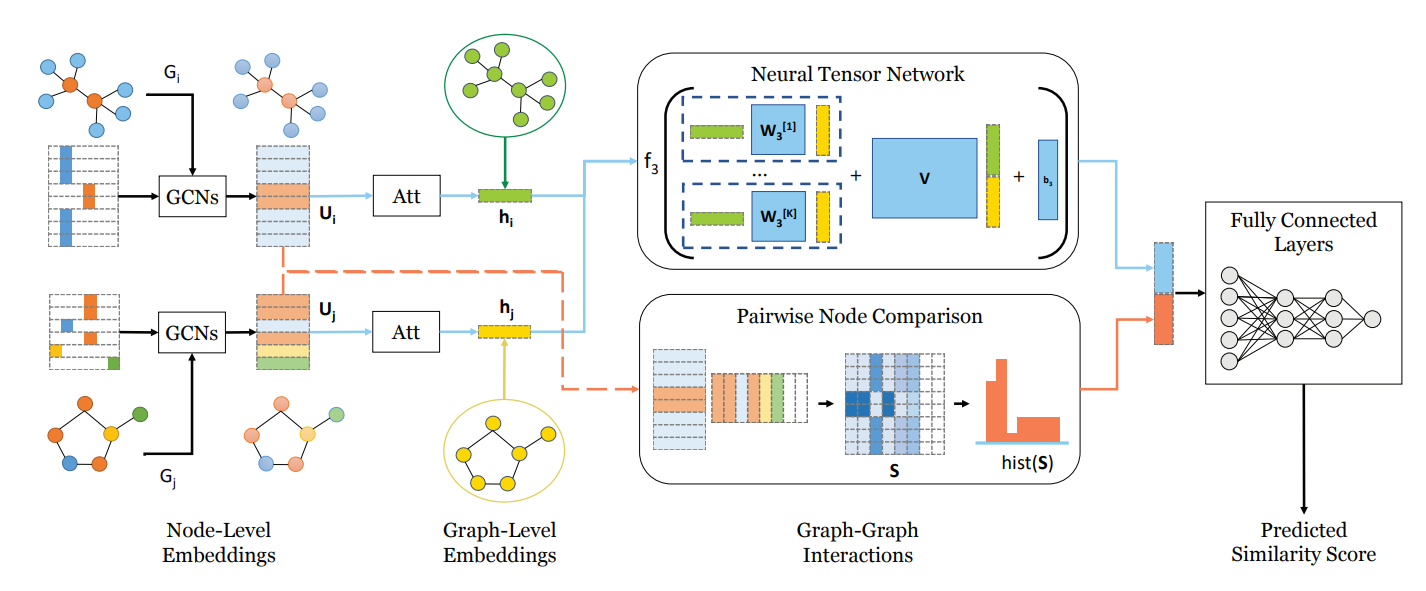
\includegraphics[width=\textwidth]{Images/simgnn_architecture.png}
		\caption{SimGNN architecture overview.}
		\label{fig:simgnn_architecture}
	\end{figure}

	
	\subsection{GPN}
	
	The Graph Path Networks (GPN) model, proposed in 2022 within the \textit{NOAH Framework} \cite{noah__neural_optimized_a*_search_algorithm_for_graph_edit_distance_computation}, introduces a novel approach to computing approximate Graph Edit Distance (GED) by leveraging the A* search algorithm optimized through neural networks. This method addresses several limitations found in previous models, including SimGNN, by improving both the search direction and search space optimization.
	
	An overview of GPN is illustrated in \autoref{fig:gpn_architecture}. The architecture of GPN comprises several key components:
	
	\begin{itemize}
		\item \textbf{Pre-training Module}: This module computes pre-training information such as exact GEDs and graph edit paths. It generates (sub)graph pairs used in training, enriching the model's understanding of graph transformations.
		\item \textbf{Graph Embedding Module}: Utilizing the Graph Isomorphism Network (GIN), this module transforms each node into a vector encoding its features and structural properties. It incorporates cross-graph information and employs an attention mechanism to obtain the final graph-level embeddings.
		\item \textbf{Learning Module}: This component focuses on optimizing the A* search algorithm by learning an estimated cost function and an elastic beam size. The estimated cost function helps guide the search direction, while the beam size adapts to various user settings, improving the search space optimization.
	\end{itemize}
	
	GPN’s enhancements over SimGNN include improved search efficiency and accuracy in GED computation. It also facilitates tasks such as graph similarity search and graph classification, demonstrating its versatility and robustness. Notably, GPN is capable of finding an edit path between graphs, utilizing a combination of pre-training information and adaptive search strategies to achieve high performance across different datasets.
	
	\begin{figure}[H]
		\centering
		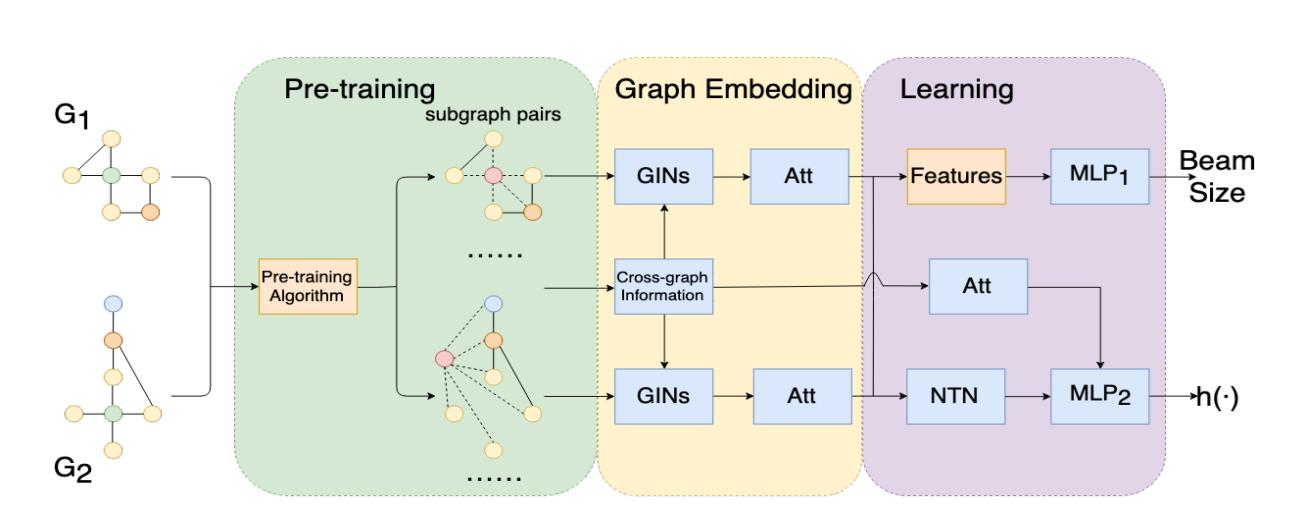
\includegraphics[width=\textwidth]{Images/gpn_architecture.png}
		\caption{GPN architecture overview.}
		\label{fig:gpn_architecture}
	\end{figure}
	
	
	\subsection{TaGSim}
	
	TaGSim (Type-aware Graph Similarity) \cite{TaGSim_type_aware_graph_similarity_learning_and_computation}, introduced in 2022, represents a significant advancement in the computation of Graph Edit Distance (GED) by addressing the limitations of previous approaches, including those that treat GED as a single global measure. TaGSim refines GED computation by considering the distinct impacts of various types of graph edit operations.
	
	An overview of TaGSim is illustrated in \autoref{fig:tagsim_architecture}. The TaGSim framework operates through the following key components:
	
	\begin{itemize}
		\item \textbf{Type-Aware Graph Embeddings}: TaGSim models the transformative impacts of four specific graph edit operations—node insertion/deletion (NR), node relabeling (NID), edge insertion/deletion (ER), and edge relabeling (EID). Each type of operation is handled separately to capture its localized effects on the graph.
		\item \textbf{Graph Edit Value (GEV) Dimensions}: GED is decoupled into four dimensions corresponding to the different types of graph edits. TaGSim estimates each dimension individually, providing a more granular and accurate representation of graph similarity.
		\item \textbf{Type-Aware Neural Networks}: The framework uses neural networks that are specifically designed to process and learn from the type-aware embeddings. This allows TaGSim to achieve high accuracy in GED estimation by incorporating the distinct impacts of different edit types.
	\end{itemize}
	
	TaGSim’s approach offers several advantages over traditional GED computation methods and previous AI-based models. By decoupling the GED into different dimensions, it avoids the pitfalls of treating GED as a single undifferentiated metric. This granularity enhances both the accuracy and interpretability of the similarity scores, making TaGSim a robust solution for various graph analysis tasks.
	
	\begin{figure}[H]
		\centering
		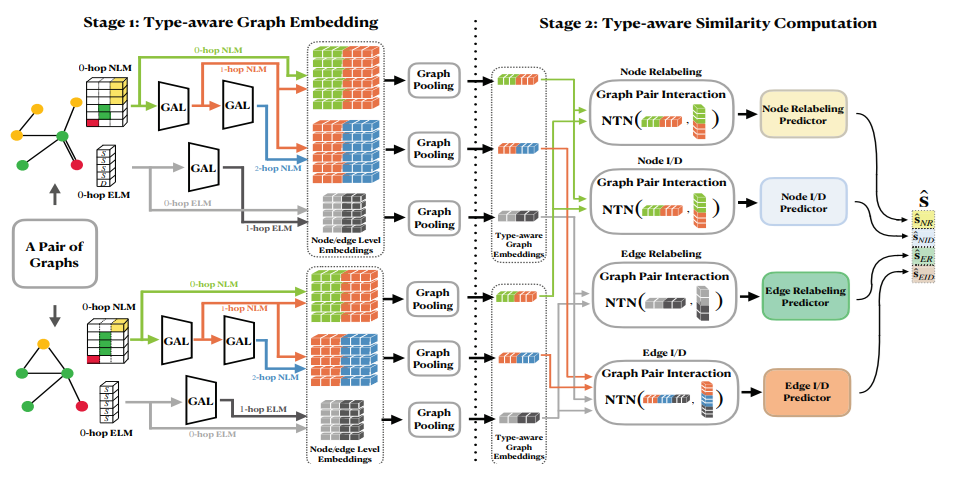
\includegraphics[width=\textwidth]{Images/tagsim_architecture.png}
		\caption{TaGSim architecture overview.}
		\label{fig:tagsim_architecture}
	\end{figure}

	\subsection{GedGNN}
	
	GedGNN (Graph Edit Distance via Neural Graph Matching) \cite{computing_graph_edit_distance_via_neural_graph_matching}, introduced in 2023, represents the latest advancement in the field of Graph Edit Distance (GED) computation. This model addresses the challenge of capturing both node and edge matching effectively through a sophisticated neural network architecture.
	
	An overview of GedGNN is illustrated in \autoref{fig:gedgnn_architecture}. The GedGNN architecture comprises several innovative components:
	
	\begin{itemize}
		\item \textbf{Graph Neural Network (GNN) Encoder}: This component uses a GNN to encode the structural and attribute information of the input graphs. The encoder generates embeddings for nodes and edges, preserving their relational information.
		\item \textbf{Node and Edge Matching Module}: This module performs node and edge matching between the two graphs. It uses an iterative matching algorithm to refine the matches, improving accuracy over multiple iterations.
		\item \textbf{k-Best Matching Post-Processing Algorithm}: To further enhance the matching accuracy, GedGNN incorporates a k-best matching algorithm. This algorithm selects the best k matching solutions from the initial matches, refining the final GED computation.
	\end{itemize}
	
	GedGNN’s comprehensive approach ensures high accuracy in GED estimation by combining robust embedding techniques with advanced matching algorithms. This model not only outperforms previous methods but also provides a flexible framework that can adapt to various types of graph structures and similarity measures.
	
	\begin{figure}[H]
		\centering
		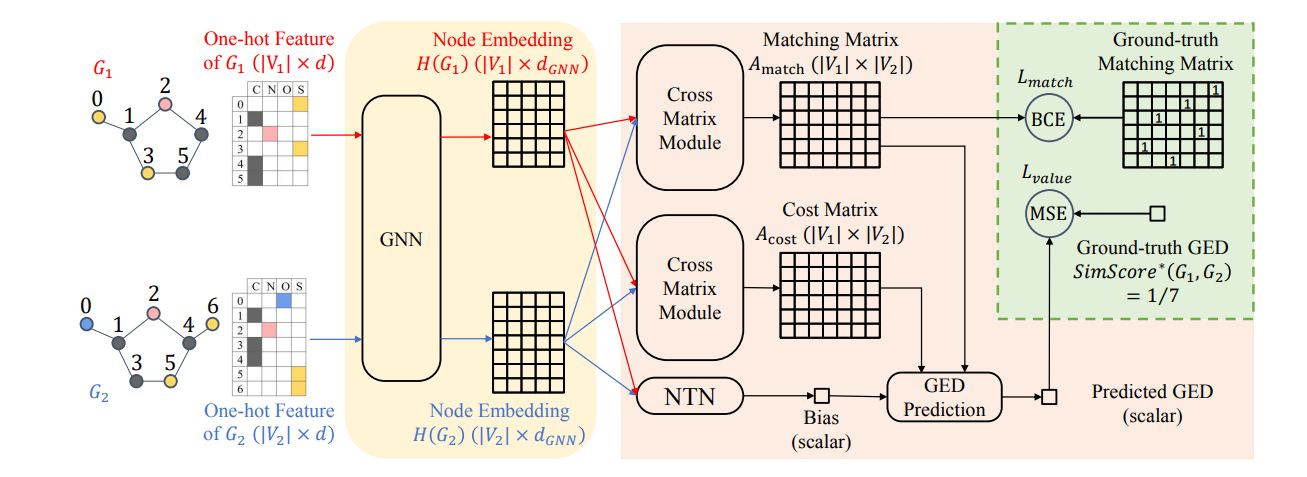
\includegraphics[width=\textwidth]{Images/gedgnn_architecture.png}
		\caption{GedGNN architecture overview.}
		\label{fig:gedgnn_architecture}
	\end{figure}
	
	\subsection{Encountered Gaps}
	
	Despite the significant advancements in graph edit distance (GED) computation, several critical gaps remain unresolved, particularly in the practical implementation and evaluation of state-of-the-art models like GedGNN \cite{computing_graph_edit_distance_via_neural_graph_matching}. One of the foremost issues is the reproducibility of results, which is severely hindered by the lack of clear and well-defined parameters. Many papers, including those on GedGNN, often provide vague instructions that make it challenging for researchers to replicate experiments accurately. Key hyperparameters, such as learning rates, regularization factors, and specific model configurations, are frequently either omitted or insufficiently detailed, leading to difficulties in achieving the reported performance when models are re-implemented or tested in different environments.
	
	Another significant gap is the poor quality of the code provided by many research works. The codebases for models like GedGNN are often poorly documented, lacking clarity and organization. This makes the code difficult to read, understand, and extend, particularly for researchers who wish to build upon these models or adapt them to new tasks. Best practices in software development, such as modular code design, comprehensive comments, and adherence to coding standards, are frequently ignored. This not only hampers reproducibility but also stifles innovation by making it harder for others to modify or improve upon the existing work.
	
	Furthermore, there are considerable concerns about the fairness of model evaluations. Many studies, including those focusing on GedGNN, employ evaluation metrics that may not fully capture the model's true performance. For instance, evaluations often rely on benchmarks that may not be representative of real-world scenarios or fail to test the model's robustness across diverse graph types and sizes. This raises the question of whether the models are genuinely being tested for their effectiveness or if the evaluations are biased towards specific datasets or problem formulations that favor the proposed models. The reliance on narrow, predefined benchmarks can lead to inflated performance claims that do not generalize well to other, more varied graph datasets.
	
	Finally, the quality of the data used for training and evaluating GED models is another significant gap. Many existing datasets suffer from several limitations, including the use of approximate GED values instead of the true edit distance, which can introduce noise and inaccuracies into the model training process. Moreover, these datasets are often small and specialized, focusing on a single type of graph application, such as chemical compound graphs or social network graphs. Consequently, models trained on these datasets tend to perform poorly when applied to different types of graphs that were not represented in the training data. This lack of generalizability is a major barrier to the broader applicability of GED models, as it suggests that the current methods are overfitting to specific data characteristics rather than learning truly generalizable patterns.
	
	In summary, while models like GedGNN represent a step forward in GED computation, significant gaps remain that hinder their practical utility and broader adoption. These gaps include challenges with reproducibility due to unclear parameters, poor code quality, unfair model evaluations, and the use of low-quality, non-generalizable datasets. Addressing these issues is crucial for the continued advancement of the field and for ensuring that GED models can be reliably and effectively applied in diverse real-world scenarios.

	
\end{document}
